%!TEX root = ../thesis.tex
\chapter{Methods}
\label{chap:methods}

\section{Extension of the SAFT information dimensionality}

\label{chap:SAFT_Augment}
One of the main objectives of this thesis is the introduction of a fourth imaging modality for the reconstruction algorithm of 3D \ac{usct} images. This modality can be used to for a classification of different tissue types by analysing the scattering characteristics of each tissue sample. 

As it was mentioned in the motivation in Section \ref{chap:motivation} the three dimensional volume of the image is extended to differentiate the directional information of the data over two additional dimensions. The three dimensional spacial information is extended by a two dimensional angular information of the emitter and receiver configuration. This approach results in a five dimensional image volume. 

The idea shall be explained by an example with Rubik's cubes:
The typical 3D reconstructed image shall be represented by a white Rubik's cube as seen in Figure \ref{3D_rubics}:
\begin{figure}[H]
    \centering
    \includegraphics[width=0.2\textwidth]{Graphics/rubicscube.png}
    \caption{Standard \ac{saft}: three dimensional spacial representation of the image as a Rubik's cube.}
    \label{3D_rubics}
\end{figure}

A \ac{saft}-image has three dimensions with the corresponding voxels which are here represented by the blocks of the Rubik's cube in Figure \ref{3D_rubics}. Each block has a voxel value $V_k$ which results from the superposition of each \ac{ascan}-sample from the \ac{saft} reconstruction. This is the standard case where no directional information is available. From this \ac{saft} representation the emitter and receiver information can not be differentiated.

The introduction of the 4th dimension helps with the preservation of directional information. Basically, the three dimensional volume of the image is split into as many parts as there are directional vectors. The directional vectors basically are a discretised form of the directional information around each voxel which helps to quantify the direction from where the signal originates or goes to. The example for four directional vectors can be seen in Figure \ref{4D_rubics}:

\begin{figure}[H]
    \centering
    \includegraphics[width=0.80\textwidth]{Graphics/rubicscube4D.png}
    \caption{The four dimensional image for a total of four directional vectors. For each directional discretisation an additional three dimensional volume is created, hence the four Rubik's cubes. The directional information is represented as the saturation of the different cubes.}
    \label{4D_rubics}
\end{figure}

The \ac{ascan} is assigned to a certain voxel in one of the four cubes. Each cube belongs to one receiver if the receiver information is stored in the 4\textsuperscript{th} dimension. If the emitter information isregarded, each cube contains the data of one emitter. Information about emitter and receiver can not be stored simultaneously. The schematic of the configuration of emitters and receivers can be seen in Figure \ref{4D_problem}:

\begin{figure}[H]
    \centering
    \includegraphics[width=0.65\textwidth]{Graphics/problem_4D.png}
    \caption{Example of imaging aperture with four receivers and two emitters.}
    \label{4D_problem}
\end{figure}

In Figure \ref{4D_problem} a simple example for four receivers and four emitters is given. The green square in the aperture represents an arbitrary voxel in a tissue sample which shall be examined. What directional information is stored in each dimension of the four Rubik's cubes depends on what configuration is of interest. One possibility would be to assign each receiver direction to a Rubik's cube. In that case the information of the emitters would be lost. In this example the emitter $e_1$ could be the emitting transducer and receiver $r_2$ the receiver. This would result in an \ac{ascan} which can be processed with the \ac{saft} as was shown in section \ref{sec:SAFT}. The resulting voxel value $V_k$ of the \ac{saft} would be assigned to the 2\textsuperscript{nd} Rubik's cube in Figure \ref{4D_rubics}. If this procedure is repeated for every \ac{ascan} there is, each voxel value would be assigned to one of the Rubik's cubes that belong to the corresponding receiver index. The information of which emitter belongs to which voxel value is lost i.e. the directional information is averaged for all emitting directions. The summation of all Rubik's cubes along this new 4\textsuperscript{th} dimension would result in the three dimensional \ac{saft} image that has no directional information and was shown in Figure \ref{3D_rubics}. 

This approach could also be used to analyse the emitter configuration which would lead to a set of Rubik's cubes that are assigned to the emitter direction. In this case the information of the receivers would be lost. 

\bigskip

A 5\textsuperscript{th} dimension can be used to keep both information about the emitter as well as the receiver. For this, the four Rubik's cubes that represent the fourth dimension are repeated into the 5\textsuperscript{th} dimension as many times as there are directional vectors. For four directional vectors this leads to $4\times 4=16$ total Rubik's cubes. An example of this is shown in the following figure:

\begin{figure}[H]
    \centering
    \includegraphics[width=0.8\textwidth]{Graphics/rubicscube5D.png}
    \caption{Example of a five dimensional set of Rubik's cubes. The information in the 4\textsuperscript{th} dimension is represented by the saturation and represents the receiver direction. The emitter information is kept in the 5\textsuperscript{th} dimension which is represented by the different colours of the cubes. 
    }
    \label{5D_rubics}
\end{figure}

In the case of four directional vectors (i.e. here four receivers or four emitters) the resulting five dimensional volume consists of 16 Rubik's cubes each containing the information in which direction the emitter lays as well as in which direction the receiving transducer was. For the example in Figure \ref{4D_problem} one possible configuration could be that emitter $e_2$ sends an ultrasound wave into the aperture. This pulse scatters at the location of the green voxel and is reflected to receiver $r_1$. The voxel value $V_k$ for this configuration would be assigned to the Rubik's cube at the coordinates $(1,2)$ in Figure \ref{5D_rubics} and would be entered at the corresponding voxel position of that particular Rubik's cube.
With this method now an arbitrary resolution of the directional discretisation can be handled. From this 5D volume the reflection characteristics of different tissue types can be plotted and compared. 


One downside of this partitioning of the \acp{ascan} into many sub-volumes is the loss of contrast in the individual images. Each Rubik's cube contains only a part of the initial 3D \ac{saft} image. Since the number of \acp{ascan} is constant each new volume receives only a fraction of the available \acp{ascan}. The overall contrast therefore is distributed between the different Rubik's cubes and therefore lower for one cube alone. 

A challenge of the additional dimension is the exponential growth of the data that has to be processed. A typical 3D volume of $250\times250\times250$ voxels contains $15.6\times10^6$ elements. Each element has a voxel value that is stored as a double value of 8 byte. For the 3D volume alone 119 MB of data have to be stored. The 5D approach increases this amount of data to 1.9 GB for only 4 directional vectors.   



\section{Discretisation of directional information}
\label{chap:segmentation}


The first step of the preservation of directional information during the reconstruction is the generation of a suitable set of directional vectors which divide each voxel volume as evenly as possible.
Theoretically, a continuous approach for the directional information could be pursued. This would lead to set of directional vectors for every voxel to every receiver and every emitter of the \ac{usct}. For this case a constant set of directional vectors would not be feasible since every voxel position affects the vectors from the voxel to the corresponding receivers and emitters. Therefore, an image volume of $250 \times 250 \times 250$ voxels with 157 \ac{tas} and each \ac{tas} containing 4 emitters and 9 receivers would lead to $1.387\times 10^{12}$ directional vectors, if 10 aperture positions are acquired. Each vector is classified by three double values which would lead to $3026.4$ terabytes of data that has to be stored solely for the vector orientations. If the actual image data would be assigned to this hypothetical set of directional vectors the storage requirements would increase manifold. Thus, a trade-off between the resolution of the discretisation and the storage requirements has to be found. To achieve that, the directional information for each voxel is discretised into a set of directional vectors. The directional vectors then are placed into the centre of each voxel facing outwards. During the reconstruction for every directional vector an individual volume is created. This was explained in section \ref{chap:SAFT_Augment}. Theoretically, the directional vectors do not have to be distributed equally. If a certain direction requires a higher resolution of the segmentation it would be no problem to either add more vectors to that particular direction or shift some existing vectors from a less relevant direction to that required direction. In the following it was aspired to distribute the vectors as evenly as possible since no information about the relevance of one certain direction over another are available during the time of writing.
Section \ref{chap:platonicsolids} explains how the properties of platonic solids can be used to generate a set of either 12 or 20 uniformly distributed vectors. The limitation of the amount of vectors which arises with the usage of platonic solids is tackled by the method of arbitrary segmentation in section \ref{chap:arbitrarySegment}.



\subsection{Platonic solids}
\label{chap:platonicsolids}

Since the goal of the segmentation is to divide the measurement volume of each voxel as evenly as possible the intermediate angle between two neighbouring segmentation vectors should be equal. Platonic solids are one possibility to get a set of vectors which fulfil this requirement and was presented by Patrick Hucker \cite{PatrickHucker2014EvaluationRuckstreumodells}.
\begin{figure}[H]
     \centering
     \begin{subfigure}[b]{0.19\textwidth}
         \centering
        \includegraphics[width=0.8\linewidth]{Tetrahedron.jpg}
         \caption{Tetrahedron}
         \label{fig:Tetrahedron}
     \end{subfigure}
     \hfill
     \begin{subfigure}[b]{0.19\textwidth}
         \centering
         \includegraphics[width=0.87\textwidth]{cube.jpg}
         \caption{Cube}
         \label{fig:cube}
     \end{subfigure}
     \hfill
     \begin{subfigure}[b]{0.19\textwidth}
         \centering
         \includegraphics[width=0.8\textwidth]{280px-Octahedron.jpg}
         \caption{Octahedron}
         \label{fig:Octahedron}
     \end{subfigure}
     \hfill
     \begin{subfigure}[b]{0.19\textwidth}
         \centering
         \includegraphics[width=0.93\textwidth]{280px-Dodecahedron.jpg}
         \caption{Dodecahedron}
         \label{fig:Dodecahedron}
     \end{subfigure}
     \hfill
     \begin{subfigure}[b]{0.19\textwidth}
         \centering
         \includegraphics[width=0.8\textwidth]{280px-Icosahedron.jpg}
         \caption{Icosahedron}
         \label{fig:Icosahedro}
     \end{subfigure}
        \caption{The five platonic solids. They all have equally sized faces. Source: \cite{wiki_platonic}}
        \label{fig:platonic_solids}
\end{figure}

A key feature of platonic solids are the equally sized faces and therefore the evenly distributed face normals if placed in the centre of each face.
There are five different platonic solids (shown in Fig. \ref{fig:platonic_solids}): The tetrahedron with four faces, the cube with six faces, the octahedron with eight faces, the dodecahedron with 12 faces and the icosahedron with 20 faces.
From these five platonic solids the dodecahedron as well as the icosahedron have previously been used to generate suitable segmentation vectors. Theoretically, the remaining geometries provide a suitable set of evenly distributed normals for the segmentation of the volume as well. Since they only have eight or less faces the comparably low resolution of the segmentation of the volume would make an analysis of the direction of propagation rather difficult.

\bigskip

Figure \ref{fig:Dodecahedron_MATLAB} shows the implementation of the dodecahedron in MATLAB. Each face normal as well as the corresponding index is plotted in the centre of each face.

\begin{figure}[H]
     \centering
     \begin{subfigure}[b]{0.47\textwidth}
         \centering
        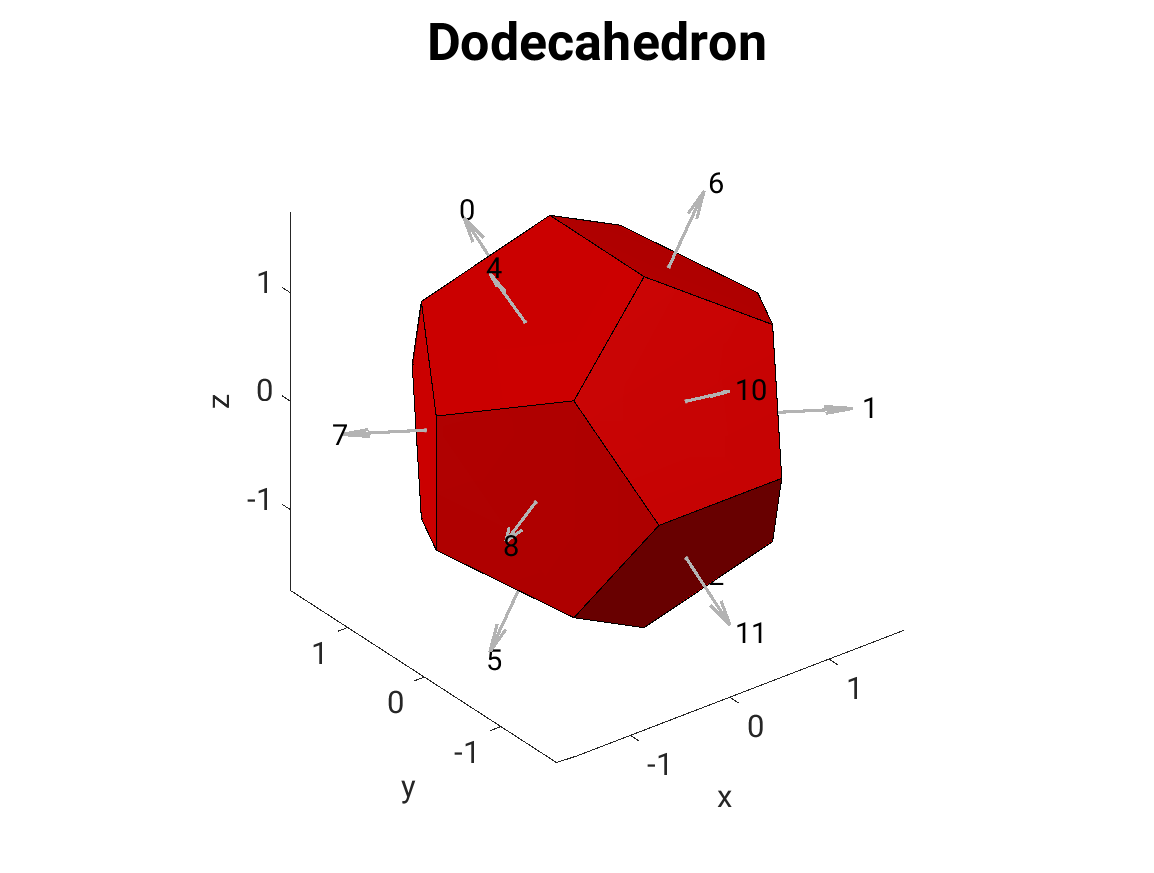
\includegraphics[width=1.2\linewidth]{Graphics/Dodecahedron.eps}
         \caption{Dodecahedron with 12 faces and 12 face normals.}
         \label{fig:Dodecahedron_MATLAB}
     \end{subfigure}
     \hfill
     \begin{subfigure}[b]{0.47\textwidth}
         \centering
         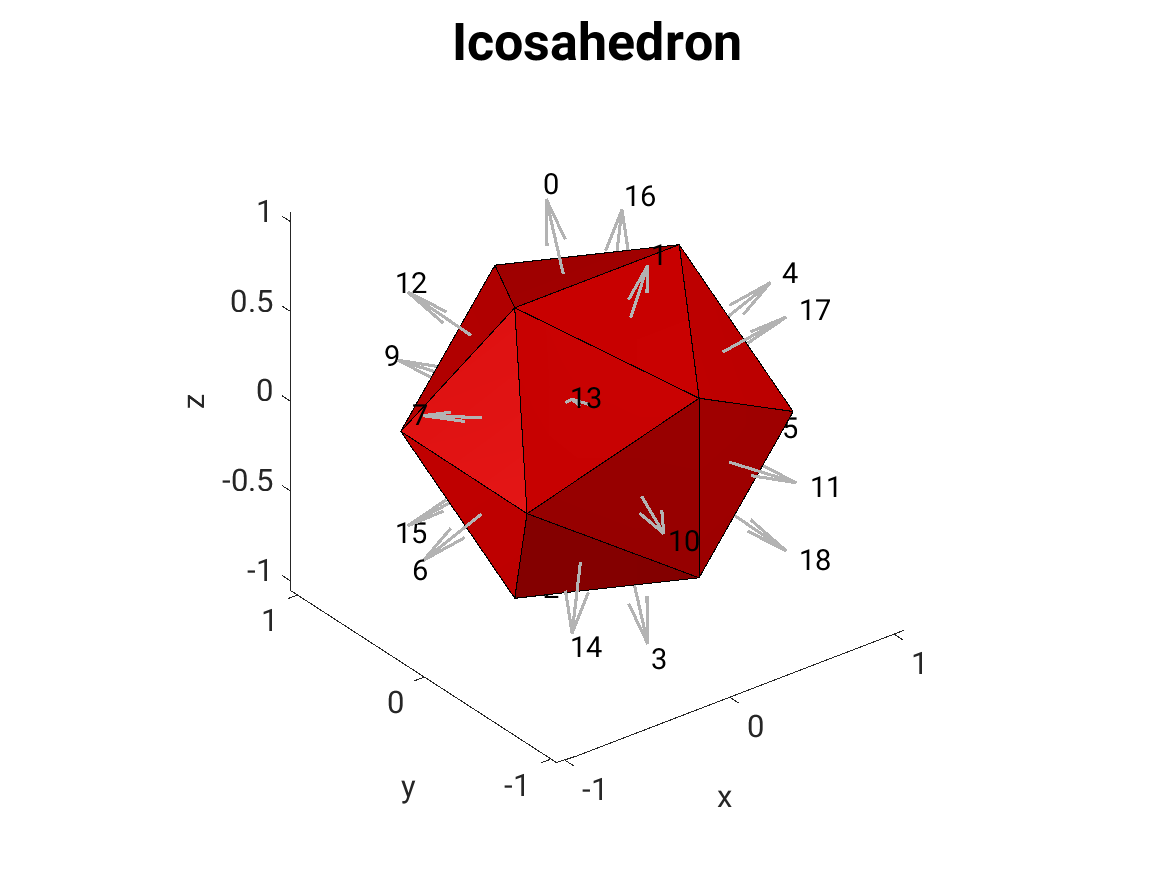
\includegraphics[width=1.2\textwidth]{Graphics/Icosahedron.eps}
         \caption{Icosahedron with 20 faces and 20 face normals.}
         \label{fig:Icosahedron_MATLAB}
     \end{subfigure}
        \caption{Both platonic solids realised in MATLAB. In the centre of each face the normal vector is plotted with its corresponding index. }
        \label{fig:platonic_solids_matlab}
\end{figure}


\subsection{Arbitrary directional segmentation}
\label{chap:arbitrarySegment}

The reflection characteristic of a medium depends on the angle under which an incoming ultrasound wave is scattered and reflected. To distinguish between very narrow angles for specular reflections and the broader angles in the diffuse case the directional information has to be given in a sufficient resolution. If the resolution of the platonic solids is not sufficient to distinguish between specular and diffuse reflectivity there has to be a way to increase it arbitrarily.
This is why one fundamental part of this thesis was the augmentation of the method for the generation of suitable directional vectors to discretise the directional information arbitrarily in contrast to the fixed number of normals that were yielded by the platonic geometries. To be able to increase the density of the segmentation vectors it is necessary to create an arbitrary amount of them. The challenging part is the alignment of the directional vectors so that every neighbouring vector has a similar angle to its other neighbours.
The problem of generating a set of uniformly distributed vectors is known as the Thomson Problem \cite{Thomson1904OnStructure}. It was formulated as the problem of the minimisation of the electro-static potential energy of $N$ equally charged particles located on the surface of a unit sphere. The particles were all equally charged and therefore repel each other following Coulomb's Law. The equation for the Coulomb potential is shown in Equation \ref{Coulombslaw} for two charged particles $i$ and $j$:
\begin{equation}
\Phi(r_{i,j}) = \underset{=k_e}{\underbrace{\frac{1}{4\pi\varepsilon_0}}} \frac{q_i \, q_j}{r^2} =  k_e \frac{q_i \, q_j}{{|r_{i,j}|}^2} 
\label{Coulombslaw}
\end{equation}
With $|r_{i,j}|$ being the Euclidean distance between two charged particles with the charges $q_i$ and $q_j$. $k_e$ is the electrostatic constant. Assuming that both particles are equally charged ($q_i = q_j = 1$) the equation for the electrostatic potential energy can be simplified:
\begin{equation}
\Phi(r_{i,j}) = \frac{k_e}{{|r_{i,j}|}^2} 
\label{Coulombslaw_simple}
\end{equation}

The combination of a set of $N$ charged particles results in the following potential:

\begin{equation}
\Phi(r_{i,j}) = k_e \sum_{i = 1}^{N}\sum_{i \neq j}^{}\frac{1}{{|r_{i}-r_{j}|}^2} 
\label{Coulombslaw_simple_set_n}
\end{equation}


The optimisation problem can be expressed as a penalty function with the so-called Reisz s-energy $\varepsilon_s (r_{i,j})$ as seen in Equation \ref{riesz_energy}. The goal is the minimisation of the Reisz s-energy by the means of maximising of the distance between the particles \cite{EtayoMinimizinSpehres}:

\begin{equation}
min\, \varepsilon_s (r_{i,j}) = min\, \sum_{i = 1}^{N}\sum_{i \neq j}^{}\frac{1}{{|r_{i}-r_{j}|}^s}
\label{riesz_energy}
\end{equation}

In Equation \ref{riesz_energy} $s$ is the the Reisz s-energy parameter which defines the penalty for the smallest distance between two points. This means that with higher $s$ the optimisation algorithm will try to the maximise the overall distance between the points to reach a better solution compared to lower $s$ values. This comes with the downside of increased computational expense. Furthermore, $k_e$ can be neglected since it is constant and does not have an influence on the solution of the optimisation problem. The actual solution for this optimisation problem can be found by applying numerical approaches like the line search algorithm.

\medskip

For the calculation of the final point configuration the implementation from \cite{AntonSemechkoSuiteSphere} was used. The result is an approximately uniform triangular configuration of points on a sphere for a set of $N$ electrically charged particles. The algorithm itself does not make use of a line search algorithm. Instead it distributes the particles in a random manner and uses thresholds to decide if a new configuration yields a better solution of the optimisation problem than the one before. Then new constraints are defined and the particles are again distributed randomly until they fall below a threshold. This is repeated until a given quality of the optimisation is reached. Figure \ref{fig:arbitrary_example} shows four examples for the resulting set of $N$ equally distributed points on the sphere.

\begin{figure}[H]
     \centering
     \begin{subfigure}[b]{0.4\textwidth}
         \centering
        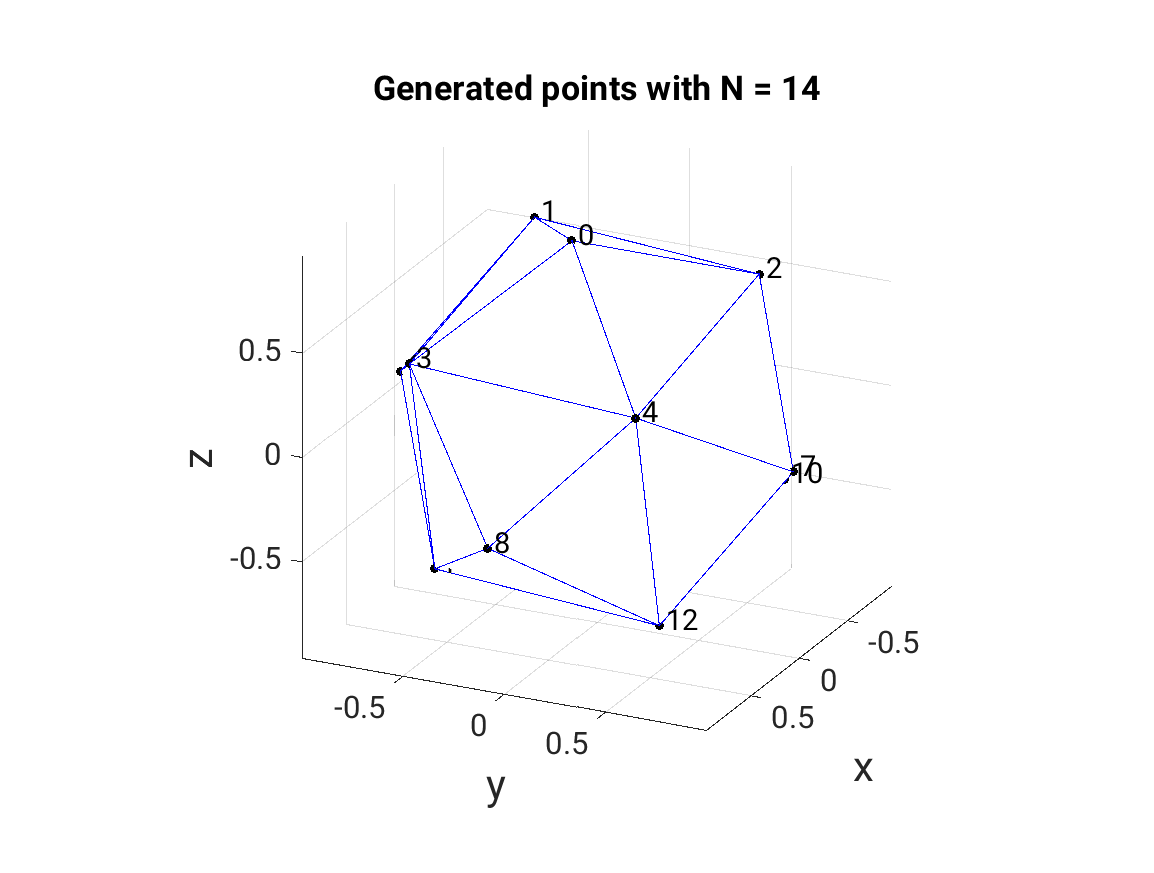
\includegraphics[width=1.3\linewidth]{arbitrary_nomals14.eps}
         %\caption{Configuration for $N = 14$ points.}
         \label{fig:arbitary_n14}
     \end{subfigure}
     \hfill
     \begin{subfigure}[b]{0.4\textwidth}
         \centering
         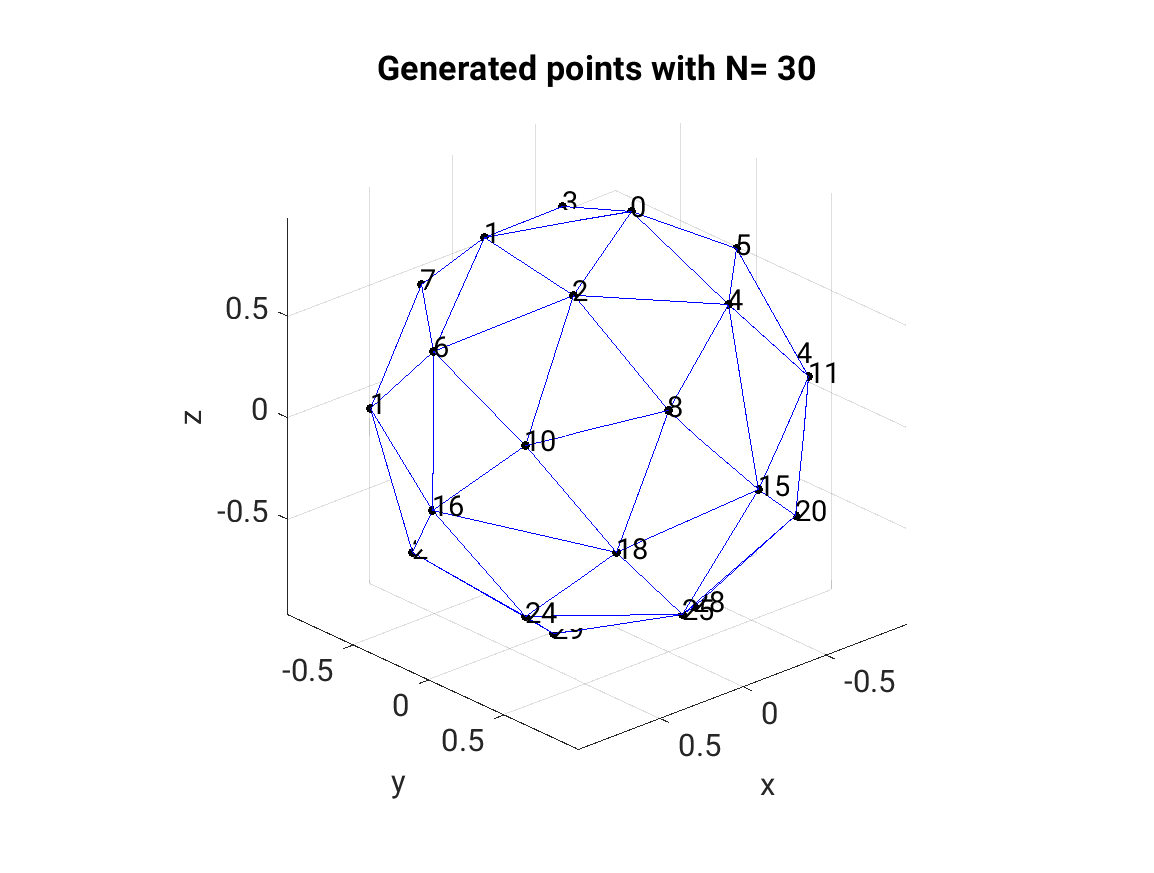
\includegraphics[width=1.3\textwidth]{Graphics/arbitrary_nomals30.eps}
         %\caption{Configuration for $N = 30$ points.}
         \label{fig:arbitary_n30}
     \end{subfigure}
         \hfill
     \begin{subfigure}[b]{0.4\textwidth}
         \centering
         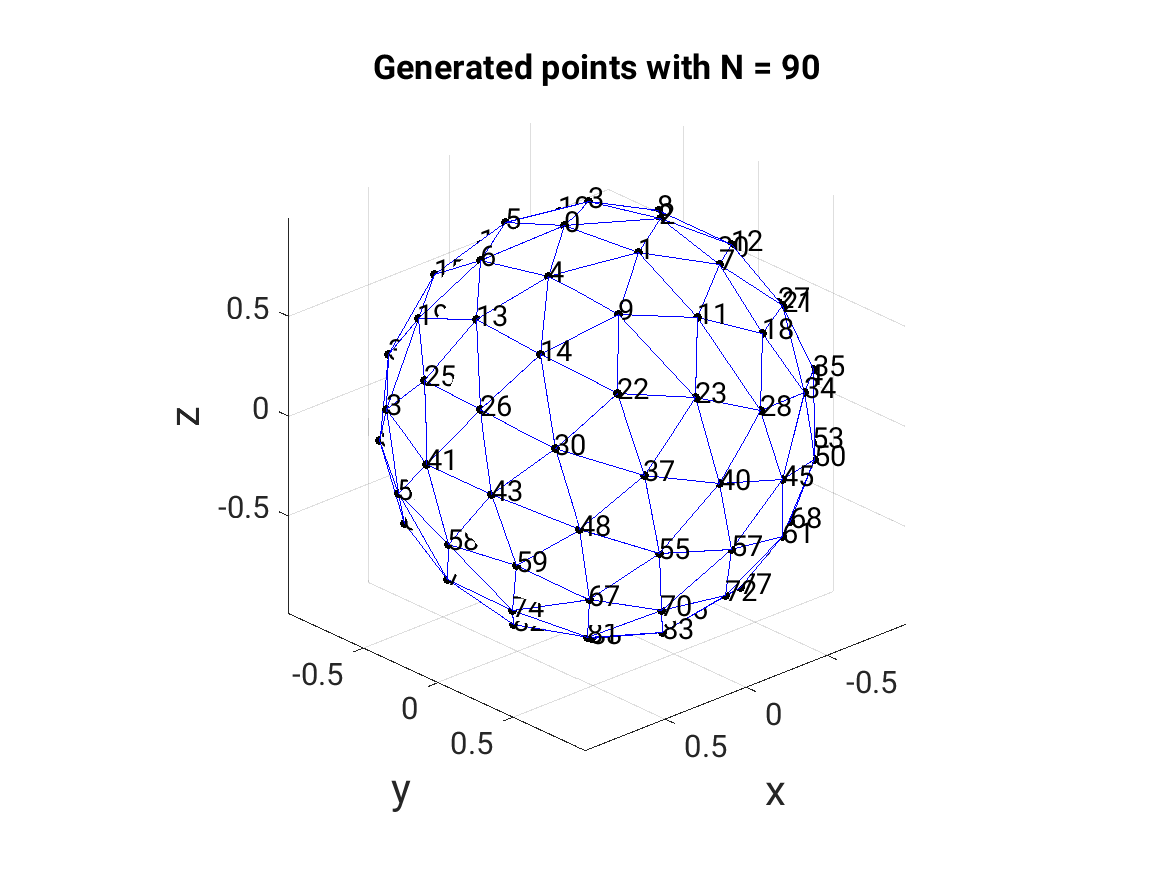
\includegraphics[width=1.3\textwidth,left]{Graphics/arbitrary_nomals90.eps}
         %\caption{Configuration for $N = 90$ points.}
         \label{fig:arbitary_n90}
     \end{subfigure}
         \hfill
     \begin{subfigure}[b]{0.4\textwidth}
         \centering
         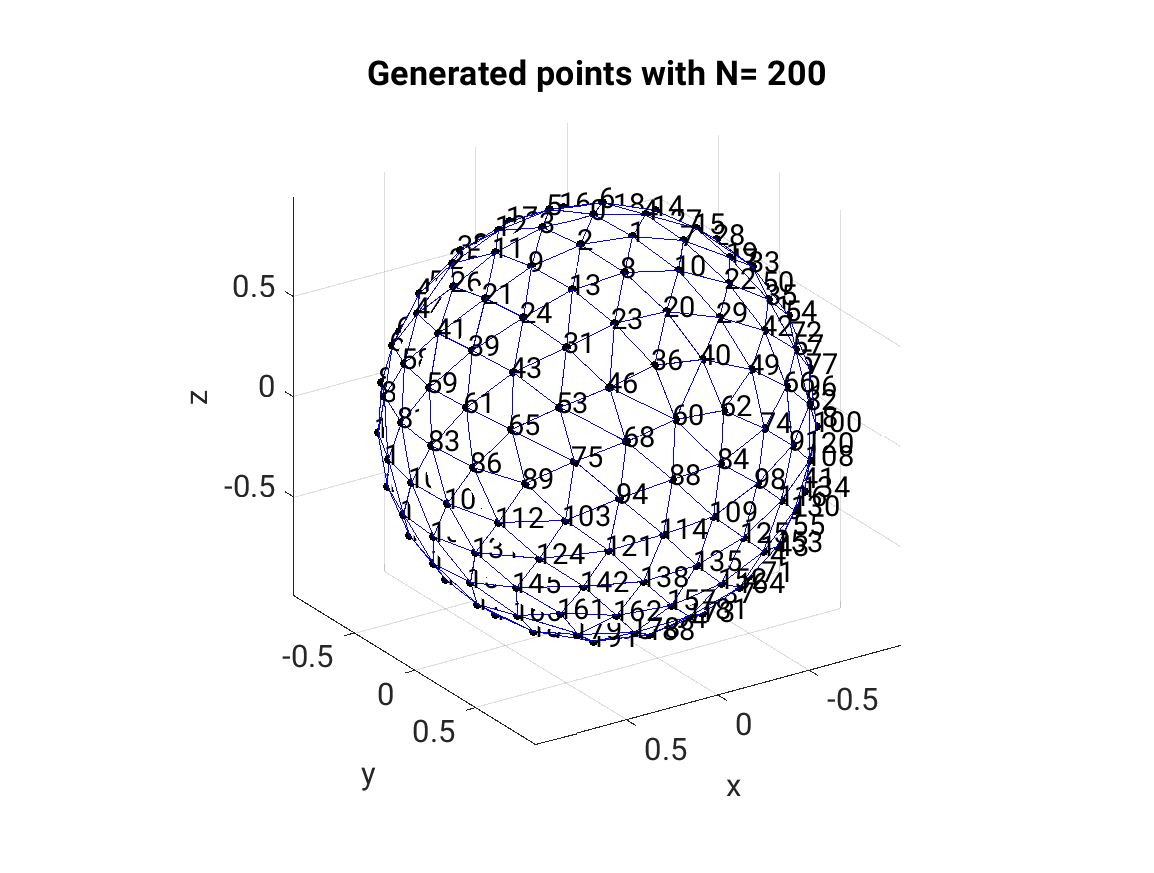
\includegraphics[width=1.3\textwidth]{Graphics/arbitrary_nomals200.eps}
         %\caption{Configuration for $N = 200$ points.}
         \label{fig:arbitary_n200}
     \end{subfigure} 
        \caption{With the arbitrary directional segmentation approach it is possible to generate an arbitrary set of equally spaced points on the surface of a sphere which then can be used to create the vectors to segment the volume. }
        \label{fig:arbitrary_example}
\end{figure}

From this triangular tessellation it is possible to derive a set of vectors which segment the measurement volume. The start point of each vector is chosen as the centre of a voxel. The vectors then are constructed to the points of the tessellation. The indexes on the points represent the order in which they were generated. A physical context can not be derived from the enumeration.  This is exemplified for $N = 14$ vectors in Figure \ref{vectors_from_points}:

\begin{figure}[H]
    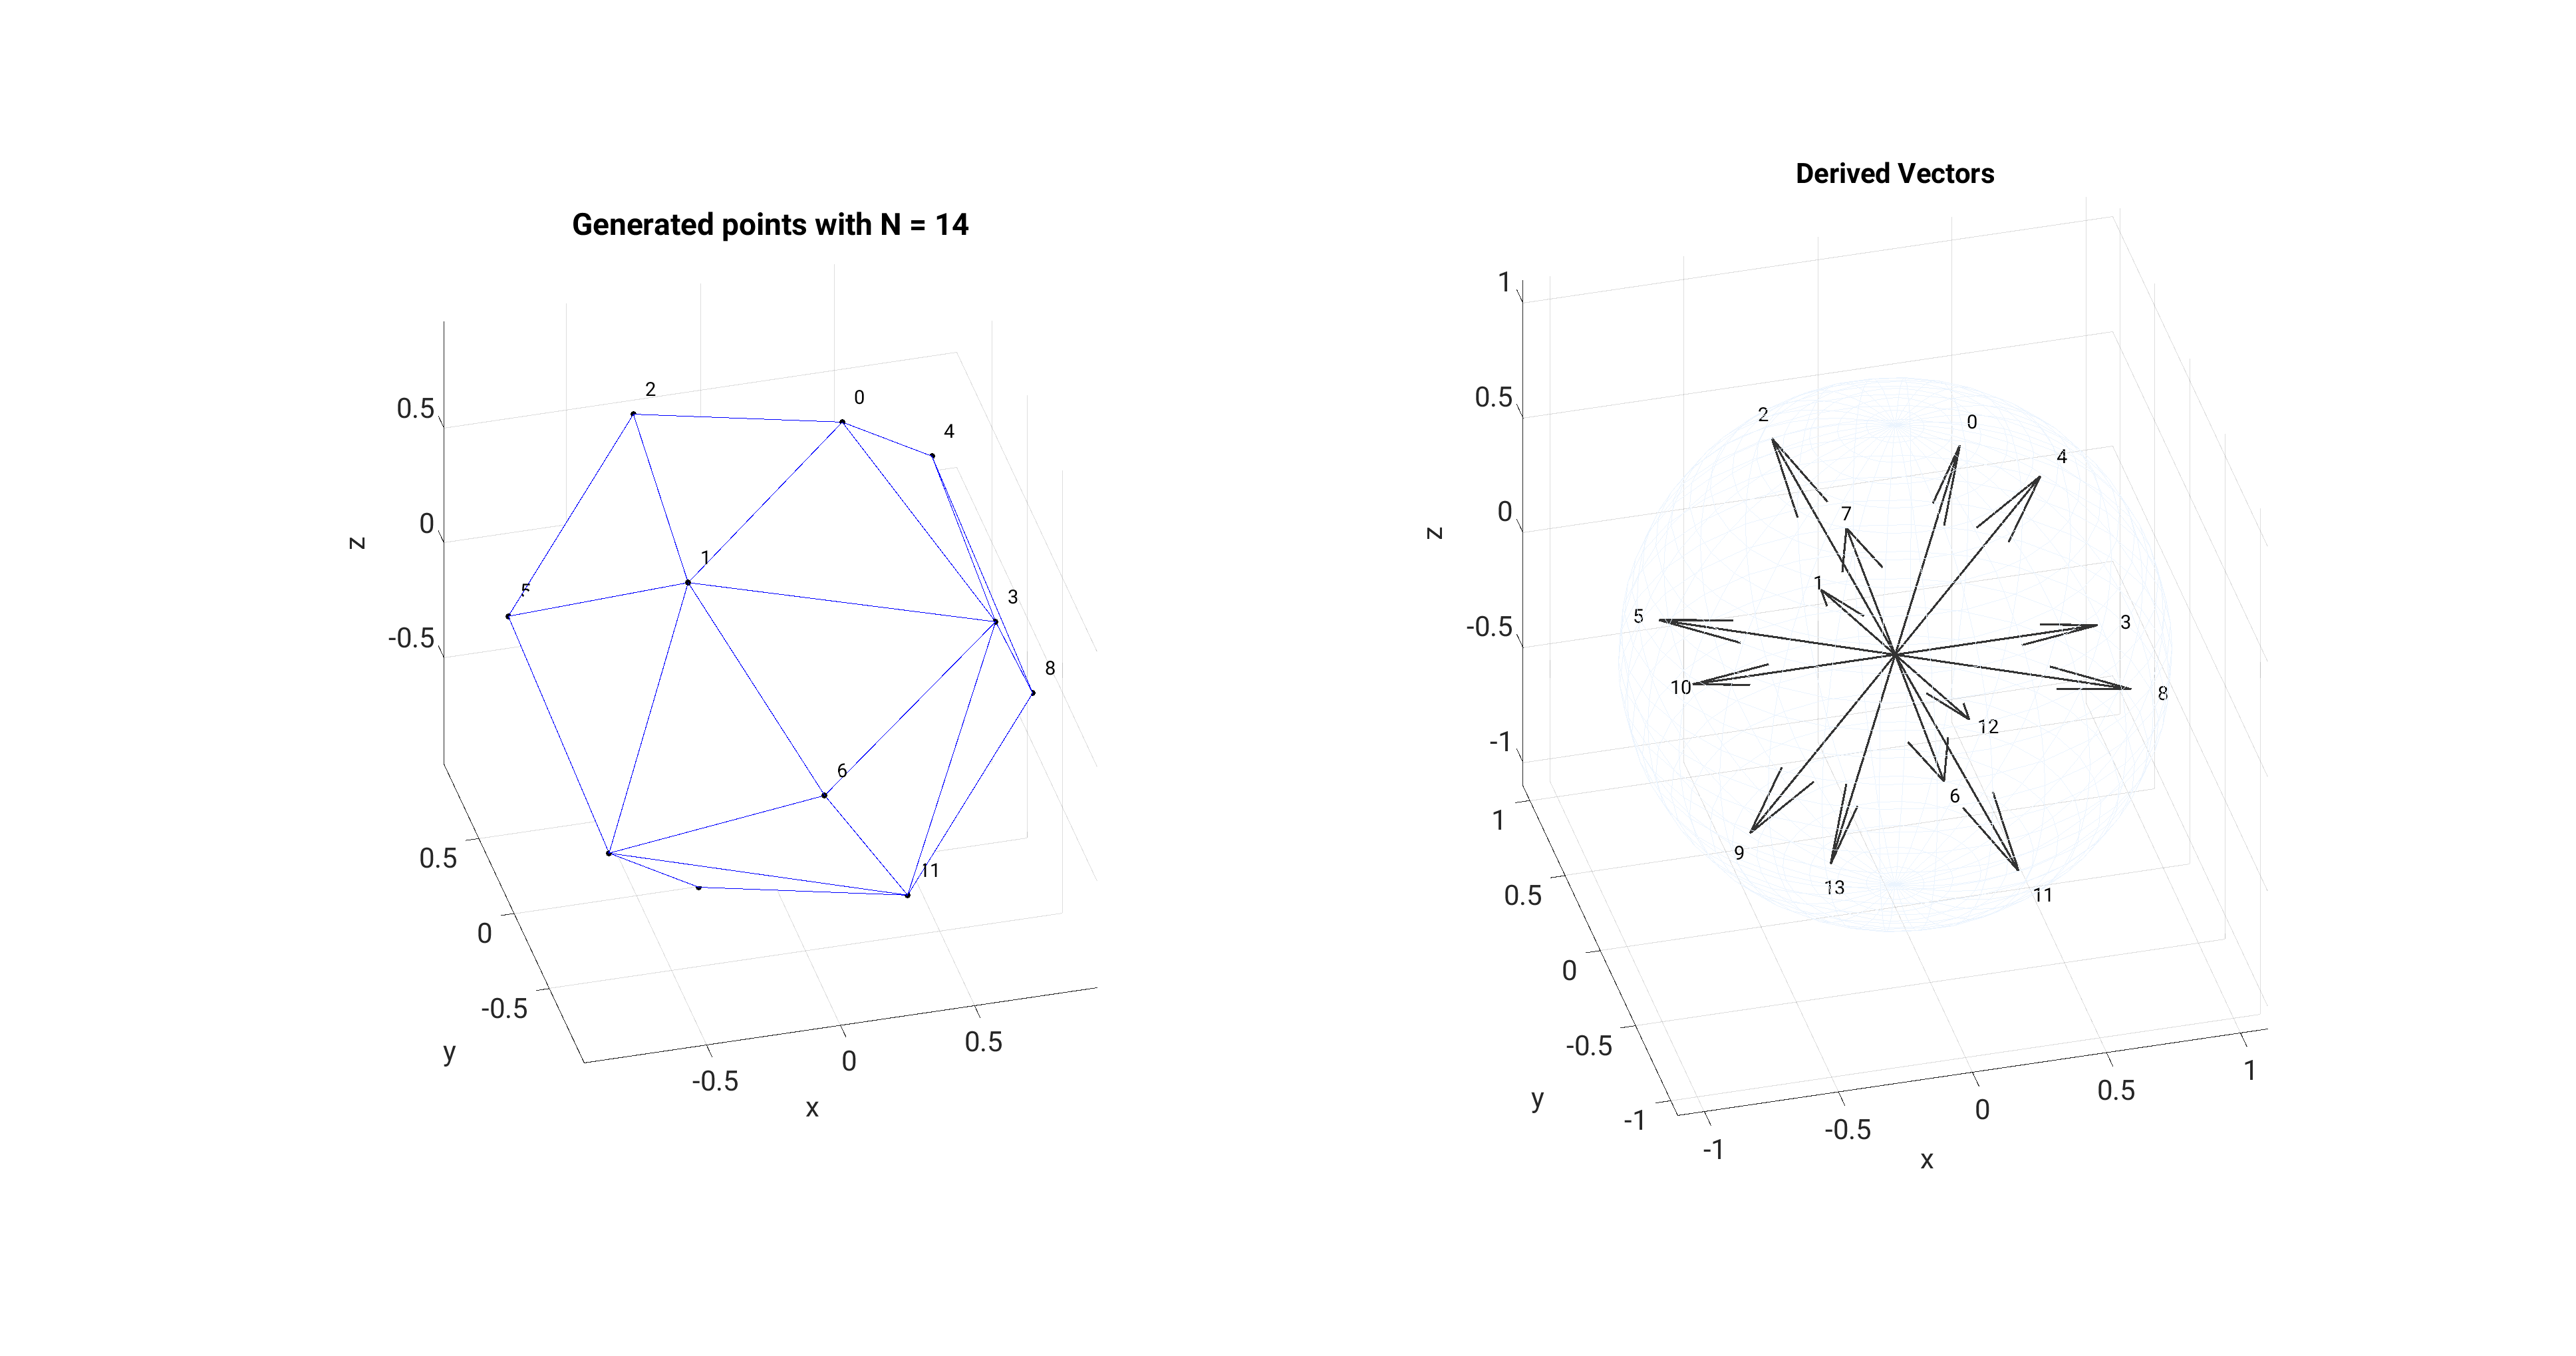
\includegraphics[width=1.39\textwidth,center]{arbitrary_nomals14_plus_vectors.eps}
    \caption{Left: A distribution of $N = 14$ points which equals Figure \ref{fig:arbitrary_example} in the top left. Right: The derived origin vectors for those 14 points.}
    \label{vectors_from_points}
\end{figure}


Since the algorithm primarily assigns each point to a random position the results would be non-reproducible. Therefore, the seed of the random number generator was set to one for each iteration so that the resulting set of points would lead to the generation of comparable vectors. 

The numerical solutions of the Thomson Problem with different numbers of particles comes to the conclusion that the minimisation of the energy results in the particles taking the form of known polyhedra. Depending on the number of charged elements $N$ different polyhedra can be expected. For $N = 4$ the minimisation of the energy results in the alignment of the electrically charged particles in the form of a tetraeder. For example for $N = 6$ they will form an octaeder and with $N = 12$ they will approximate an icosaeder. These forms are part of the platonic solids that were introduced in chapter \ref{chap:platonicsolids}. Thus, it does not make sense to generate a uniform distribution for $N = 12$ and $N = 20$ particles as we can reach these results in a much more efficient way by utilising the geometry of the platonic solids. Nevertheless, the implementation allows any number of $N > 2$ particles to find an optimal solution even if the platonic solids provide a more efficient alternative for certain numbers of particles.


\section{Comparison vectors}
\label{sec:comp_vect}

The \ac{saft} reconstructions results in a value $V_k$ for a particular voxel. The discretisation of the directional information now allows for the voxel value to be assigned to a certain directional vector. Each volume of the final image for each directional vector will be assigned only to those voxel values that belong to that directional index.
To assign a certain voxel value $V_k$ to each of the directional vectors' indices a comparison vector has to be defined for that \ac{ascan}. For this thesis mainly the comparison vectors comprise the vector from the position of the voxel which is analysed in that certain step to the position of the receiving transducer:

\begin{equation}
\vec{V}_{comp,vox\_rec} = \begin{bmatrix}
X
\\
Y 
\\
Z 
\end{bmatrix}_{rec}
-
\begin{bmatrix}
X
\\
Y 
\\
Z 
\end{bmatrix}_{vox}
\label{comp_vect}
\end{equation}

and the vector from the voxel position to the emitter:

\begin{equation}
\vec{V}_{comp,vox\_emit} = \begin{bmatrix}
X
\\
Y 
\\
Z 
\end{bmatrix}_{emit}
-
\begin{bmatrix}
X
\\
Y 
\\
Z 
\end{bmatrix}_{vox}
\label{comp_vec2t}
\end{equation}

It is essential to normalise the comparison vectors as well as to define them starting at the voxel position. In case of defining for example the directional vector from equation \ref{comp_vec2t} from the emitter to the voxel the reconstructed image would be rotated $180^{\circ}$ since the algebraic sign of the orthogonality is switched.
In previous approaches only one directional vector was used. The reason for that was the assumption of a specular reflectivity model of the tissue which was mentioned in section \ref{sig:flect_character}. The usage of two different directional vectors for the emitter-voxel relation as well as for the receiver-voxel relation makes it possible to actually analyse the reflection characteristics of the tissue. For the receiver and emitter a new dimension of the reconstructed image is introduced which allows for the sampling of the reflection characteristic of each voxel and quantify the specular and diffuse parts in the reflection. The result is a five dimensional image with all the directional information stored in one of the arrays as it was explained in section \ref{chap:SAFT_Augment}. This potentially leads to a higher diagnostic value of the tissue classification than the previous case.



\section{General procedure for calculating directional information}
\label{chap:algo_for_direction_recon}

Figure \ref{Basic_Algo_Angle_ident} shows the general procedure of reconstructing an \ac{usct} image with directional information. The flowchart shows the algorithmic description of the assignment process that was exemplary described in section \ref{chap:SAFT_Augment} with the Rubik's cubes. The stages in grey originate from the previous implementations whereas the stages in colour contain mostly new or extended approaches for the reconstruction. 

The old implementation lacked to possibility to generate 5D images. Memory limitations were one of the main reasons that the 5\textsuperscript{th} dimension could not be regarded. This limitation was overcome with the new implementation of the reconstruction.

The first stage of the flow chart is the \textbf{start of the reconstruction}. This step summarises all the preprocessing requirements of the \ac{saft} for example the quality evaluation of each \ac{ascan} and the identification of suitable receiver-emitter-configurations.
After the preprocessing the measurement volume is segmented by \textbf{generating a set of directional vectors}. This procedure of setting up the directional vectors is explained in section \ref{chap:segmentation}. At this point theoretically any vector in the voxel could be assigned to an directional vector. 

Then, with the directional vectors and a suitable set of \acp{ascan} it is possible to start with the assignment loop. The loop begins with the first \ac{ascan} (\code{AScan[0]}) and the first directional vectors for the 4\textsuperscript{th} and the 5\textsuperscript{th} dimension (\code{directional vector4D[0]} and \code{directional vector5D[0]}). 

The \textbf{\ac{saft}} section of the flow chart considers each of the \acp{ascan} and calculates a voxel value $V_k$ as it was explained in section \ref{sec:SAFT}. During this process also the speed of sound correction explained in section \ref{sec:sos_correct} is taken into account, which leads to an overall increased contrast and resolution of the final image.  

The stage following the \ac{saft} covers the process of deciding on a so-called \textbf{comparison vector} for each iteration of the loop. Section \ref{sec:comp_vect} gives more details on that step.


The central part of the reconstruction is implemented in the 5\textsuperscript{th} stage. In this stage the directional information for each \ac{ascan} is analysed and the voxel value $V_k$ assigned to the correct voxel in the corresponding dimensions. The previous implementation was heavily constricted by memory requirements and its  execution time. A new method is introduced in section \ac{chap:ortho_threshold} which overcomes these restrictions and allows for the processing of the directional information in 5D.   

After the assignment of the voxel value $V_k$ to the suitable directional index the process of calculating a voxel value $V_k$ and determining a comparison vector starts anew with the next \ac{ascan}.
Since all the calculations have to be repeated for every directional vector, once arrived at the last \ac{ascan} the next directional vector for the 4\textsuperscript{th} dimension is loaded and the whole process repeats itself. After all \code{directional vector4D} were processed the outer loop selects the next \code{directional vector5D} and the algorithm starts from the \ac{saft} stage again. Since there are multiple repeated executions of the same functions in this algorithm it is important to optimise each calculation step as much as possible. 



\begin{figure}[H]
    \centering
    \includegraphics[width=1.13\textwidth]{Graphics/AngleIndex_Algorithm.png}
    \caption{Flow chart of the algorithm for the reconstruction of an \ac{usct} image while preserving directional information in the data.}
    \label{Basic_Algo_Angle_ident}
\end{figure}





\newpage

\section{Assignment to the directional dimensions}
\label{sec:index_ident}

With the methods explained in section \ref{chap:segmentation} we receive a set of directional vectors which divide our measurement volume in an uniform manner. 
Furthermore, with the methods from section \ref{sec:comp_vect} one obtains two comparison vectors for each \ac{ascan} in the five dimensional case. The \ac{saft} reconstruction results in a voxel value $V_k$ that results from this emitter-receiver-configuration. The next step is the identification of a feasible directional vector for each \ac{ascan} and the assignment of the voxel value $V_k$ to this vectors index. Two different methods will be presented: the angle sorting method which was adapted from Patrick Hucker \cite{PatrickHucker2014EvaluationRuckstreumodells} and a novel approach, the orthogonality threshold. Both methods will be called for every \ac{ascan}, for every possible directional vector in 4D and also for every directional vector in 5D. The assignment of the directional index to the comparison vector takes place in the dotted stage of the reconstruction algorithm which is shown in Figure \ref{Basic_Algo_Angle_ident}. First it shall be shown that the orthogonality is a good metric to find the closest angle between multiple vectors and how to use it in both methods to assign a directional index to the comparison vectors. 

\subsection{Orthogonality}
\label{sec:orthogonality}

To assign each \ac{ascan} to a certain direction the orthogonality provides a good metric since it is independent of the azimuthal rotation between two vectors $\overrightarrow{a}$ and $ \overrightarrow{b}$. 
To get a conclusive result concerning the angular relation of two vectors one requirement of this method is that every vector has to be normalised. If this requirement is met one can arrive at the definition of perpendicularity:

Two vectors $\overrightarrow{a}$ and $\overrightarrow{b}$ are considered orthogonal to each other if the following assumption is fulfilled:

\begin{equation}
\overrightarrow{a} \perp  \overrightarrow{b} \Leftrightarrow  \overrightarrow{a} \cdot  \overrightarrow{b} = 0
\label{equation_orthogonality}
\end{equation}

Since this case only covers the case of an exact right angle between both vectors it is important to have a look at the the distribution of the orthogonality between the vectors $\overrightarrow{a}$ and $\overrightarrow{b}$ for different angles. An example is shown in Figure \ref{orthogonaltiy_figure}. Vector $\overrightarrow{a} = \begin{bmatrix} 0 \\ 1 \end{bmatrix}$ is represented by the green arrow on the left side. It serves as a constant reference vector. On the right side there are shown three possible vectors $\overrightarrow{b}$.

\begin{figure}[H]
    \centering
    \includegraphics[width=0.8\textwidth]{Graphics/orthogonality.png}
    \caption{Example for the calculation of the orthogonality of one static reference vector$\overrightarrow{a}$ on the left side and three possible candidates for $\overrightarrow{b}$ on the right. The calculation shows the transition of the orthogonality from its minimum of $-1$ to the maximum of $1$.}
    \label{orthogonaltiy_figure}
\end{figure}

The calculations on the right side of Figure \ref{orthogonaltiy_figure} show the orthogonality between each combination of $\overrightarrow{a}$ and $\overrightarrow{b}$. For example vector $\overrightarrow{a}$ and the purple vector $\overrightarrow{b}$ are perpendicular to each other. The calculations show that the orthogonality between both is zero and therefore fulfil the requirement of Equation \ref{equation_orthogonality}. The red vector $\overrightarrow{b}$ and the green comparison vector $\overrightarrow{a}$ comprise an angle of $180^{\circ}$ and therefore both vectors are pointing in the exact opposite direction. This results in an orthogonality of minus one.
If the vector $\overrightarrow{b}$ is pointing in the same direction as vector $\overrightarrow{a}$ they are parallel and the orthogonality between both is one. The dotted semicircle shows the transition of the orthogonality from its minimum to its maximum. In this interval the orthogonality monotonically increases non-linearly from $-1$ to $1$. The reason for the non-linear behaviour is the correlation of the scalar product with the cosine function. The scalar product of two vectors corresponds to the cosine of the angle between those vectors. For a right angle ($90^{\circ}$) the cosine becomes zero and for parallel case ($0^{\circ}$) the cosine results in one. An example of the non-linearity of the orthogonality and its relation to the cosine function is given in Figure \ref{orthogonaltiy_figure2}:

\begin{figure}[H]
    \centering
    \includegraphics[width=0.8\textwidth]{Graphics/orthogonality2.png}
    \caption{Example of the non-linearity of the orthogonality in the interval $[-1,1]$. }
    \label{orthogonaltiy_figure2}
\end{figure}

The orthogonality between the blue vector $\begin{bmatrix} 0 \\ 1 \end{bmatrix}$ and the purple vector $\begin{bmatrix} 1 \\ 0 \end{bmatrix}$ is zero since both are perpendicular. The normalised bisector in between is shown by the orange vector.
The orthogonality between the blue vector and the bisector is approximately $0.71$.

\medskip

An alternative derivation of the method to identify the direction vector is given in \ref{Alternative_herleitung}.

\newpage


\subsection{Angle sorting method}
\label{chap:angle_sorting}
The first method for assigning a directional index to a certain comparison vector will be explained in this chapter. It is an adaption of the angle sorting method from Patrick Hucker \cite{PatrickHucker2014EvaluationRuckstreumodells}. It was extended to the 5\textsuperscript{th} dimension. The assignment process takes place in the central stage of the flowchart shown in Figure \ref{Basic_Algo_Angle_ident}. 



\begin{figure}[H]
    \centering
    \includegraphics[width=1.12\textwidth]{Graphics/Angle_Sorting.png}
    \caption{Flowchart of the angle sorting algorithm.}
    \label{angle_sorting_flow}
\end{figure}

The basic approach for the successful assignment of a voxel value to the correct directional vector is finding the directional vector which is closest to the comparison vector of the particular \ac{ascan} and assign the voxel value to this direction. Since there are multiple directional vectors the comparison vector is compared to each one of them. As we are using the orthogonality as metric for the angular relation between two vectors the goal is to find the largest orthogonality between the comparison vector and each directional vector. For the directional vector which yielded the highest orthogonality the voxel value is assigned to this direction.

The input parameters for this approach are the \code{comparison\-\_vector4D} and \code{com\-parison\-\_vector5D} for both dimensions.
For this example they will be defined as the vector from the voxel to receiver for the \code{comparison\_vector4D} and the vector from the voxel to the emitter for  \code{comparison\_vector5D}.
The directional vectors that discretise the directional information of the volume have to be imported as well. They are regarded as input argument for the algorithm as an interleaved array of vector coordinates. 

The process of calculating the voxel value, the calculation of the comparison vectors and the assignment of these comparison vectors to the directional vectors is repeated two times for every directional vector there is. In each iteration two current directional vectors for the 4\textsuperscript{th} and 5\textsuperscript{th} dimension are given. The indices of the two directional vectors that are under investigation in that particular iteration of the reconstruction are given as \code{current\_\-direction\-\_vector4D} and \code{current\-\_direction\-\_vector5D}.

In the 2nd stage of this approach the iterators \code{i\_4D} and \code{j\_5D} are initialised. Furthermore, the variables \code{smallest\_angle4D} and \code{smallest\_angle5D} are initialised as an arbitrary small value. They will later hold the biggest orthogonality (since large orthogonality equals small angle) of the set of directional vectors to the comparison vector. The \code{angleIndex4D} and \code{angleIndex5D} are set to zero in the beginning. 

In the 3rd stage of this method the directional vectors for the first iteration \code{i\_4D = 0} are calculated. As the coordinates of the directional vectors are stored in an interleaved array, pointer operations can be used to access the coordinates. For '\code{+0}' the first coordinate of the directional vector is loaded. Analogously, the second and the third coordinates are taken from the array with '\code{+1}' and '\code{+2}'. The result is the first directional vector \code{dir\_vec4D} for the first iteration of \code{i\_4D}.

This is the point where the orthogonality comes into play. With the \code{comparison\-\_vector4D} and the first directional vector \code{dir\_vec4D} the scalar product can be calculated. The result is stored in variable \code{thisangle4D} which ultimately is nothing else but the orthogonality between the two vectors. The following step is for the decision whether this new \code{thisangle4D} is bigger than the \code{smallest\_angle4D}. If this is the case the left path is taken and the \code{angleIndex4D} is set to the current value of the iterator \code{i\_4D} and the new \code{smallest\_angle4D} is set as \code{thisangle4D}.

Since \code{smallest\_angle4D} was initialised as a very small value the first iteration will always lead to the left path which overwrites \code{smallest\_angle4D}. If the setting of a new \code{smallest\_angle4D} is done the iterator \code{i\_4D} will be incremented by one if the last directional vector was not already reached.
Again a directional vector \code{dir\_vec4D} is calculated from the coordinate array and the orthogonality is calculated and stored as \code{thisangle4D}. Once again the control structure checks if the new \code{thisangle4D} is smaller than the \code{smallest\_angle4D} that was set in the iteration before. For the case being bigger again the left path is chosen and the old \code{angleIndex4D} is replaced by the actual iterator \code{i\_4D} and the old \code{smallest\_angle4D} is replaced by the new \code{thisangle4D}. 

In case of \code{thisangle4D} not being bigger than the previous \code{smallest\-\_angle4D} at the end of the left side of the flowchart, the right path is taken. This leaves the \code{angleIndex4D} and the \code{smallest\_angle4D} unchanged.
This procedure is repeated for every directional vector there is. Upon reaching the last iteration in the variable  \code{smallest\_angle4D} there is saved the orthogonality between the \code{comparison\_vector4D} and its closest directional vector. The directional vectors index is stored in \code{angleIndex4D}. 

After comparing the the \code{angleIndex4D} with the \code{current\_\-direction\_vector4D} there are two options. 


The first is for the case that the \code{angleIndex4D} and the current \code{current\_\-direction\-\_vector4D} do not match. It was mentioned that the \code{current\_direction\-\_vector4D}, which is given as input for the algorithm, contains the index of the directional vector that is analysed for that iteration of the algorithm. This means that only feasible values for that particular \code{current\_\-direction\_vector4D} are accepted and every other direction is disregarded for that iteration. For that case of \code{angleIndex4D} not matching the \code{current\_direction\_vector4D} the algorithm will be stopped and the next \ac{ascan} will be analysed. This leads to a new \code{comparison\_vector4D} and possibly to a new \code{angleIndex4D}. 

The other option is that the \code{angleIndex4D} and the \code{current\_\-direction\_vector4D} actually are the same. This means that at least for the fourth dimension the \code{angleIndex4D} is the directional vector that is regarded for that iteration. In this case the flowchart on the right side of Figure \ref{angle_sorting_flow} will be followed. It shows exactly same procedure but this time for the 5th dimension. In the end there also is an \code{angleIndex5D} which will be compared to the \code{current\_\-direction\_vector5D}. If they coincide the directional vector \code{dir\_vec4D} will be assigned to \code{angleIndex4D} and analogously the directional vector \code{dir\_vec5D} will be assigned to \code{angleIndex5D}. From there the algorithm in Figure \ref{Basic_Algo_Angle_ident} continues with the next \ac{ascan}. 
















\subsubsection{Decision area for the angle sorting approach}

For the angle sorting approach the decision area for each directional vector is given by the geometrical boundaries of the geometrical arrangement of the directional vectors. For the cases of the platonic solids these geometries are known. An example for the dodecahedron is given in Figure \ref{decision_area_dodeca}. In that example six pentagonal faces of the dodecahedron are shown. The directional vectors are plotted in the middle of each face. The assignment of an comparison vector to a directional vector only depends on the face that would be pierced by the comparison vector. The particular face then leads to the directional vector and its index is assigned to that comparison vector. The whole area of each pentagon serves as decision area and the decision boundaries are the edges of the pentagon. Consequently, comparison vectors that pierce the face at a 'tip' where two boundaries meet have a larger angle to the actual directional vector than a comparison vector that pierces at the middle of a boundary of the same face. Still, both comparison vectors would be assigned the same index regardless of their different angles to the directional vector.



\begin{figure}[H]
    \centering
    \includegraphics[width=0.8\textwidth]{Graphics/decision_area_normal.jpg}
    \caption{2D example of the decision areas for the partial dodecahedron. Depending on what face of the geometry is pierced by the comparison vector it gets assigned the index of the corresponding directional vector of that face. The decision boundaries for each directional vector are the edges of the particular pentagon.}
    \label{decision_area_dodeca}
\end{figure}

The decision boundaries for $N \neq \left \{ 6,12,20 \right \}$ particles do not lead to any known platonic solid geometries. For those unknown cases the angle sorting algorithm also assigns the comparison vector to a particular directional vectors index but the decision boundaries are not as easy to plot in those cases.














\subsection{Orthogonality threshold method}
\label{chap:ortho_threshold}

A new method for the assignment of directional information is introduced in this chapter. Instead of comparing each individual directional vector with the comparison vector in order to search for the smallest angle between them, the new method calculates a threshold value beforehand and compares the orthogonality of the comparison vector to this threshold. A big advantage of this new approach is that it can be implemented in parallel where multiple execution units could divide the workload by only regarding a certain set of direction vectors. The previous implementation needed to be executed sequentially since every directional vector had to be regarded for the angle sorting step. 






\subsubsection{Decision area for orthogonality threshold}
\label{decison_orthonolatiy}

In the case of the generation of an arbitrary number of directional vectors generally there are no known geometries. In theory the angle sorting algorithm would also lead to a decision on each directional vector. Since this criterion is hard to verify for unknown geometries the goal is to find a new criterion for all directional vectors which lead to the same boundaries. These areas of decision are chosen to be cone shaped with the opening angle of the cones relating to the angle of the bisector between two normals. An example for that is shown in Figure \ref{decision_arbitrary_bisec}:


\begin{figure}[H]
    \centering
    \includegraphics[width=0.8\textwidth]{Graphics/decision_area_calc_bisector.jpg}
    \caption{Calculation of the bisector between the nearest neighbour of the first normal.}
    \label{decision_arbitrary_bisec}
\end{figure}

The decision areas for this method are shown in context of the decision areas of the dodecahedron. The first step to find an orthogonality threshold for the decision criterion is to find the nearest neighbour of the first directional vector by the means of orthogonality. This is shown in Figure \ref{decision_arbitrary_bisec}. The orthogonality is calculated for each combination of the first directional vector with each other directional vector in the geometry. For the pair with the highest orthogonality it can be assumed that this is the approximately nearest neighbour by means of the angle between them. Since this nearest neighbour is only searched for the first directional vector this results in an locally optimal solution. Theoretically, every combination with each directional vector has to be tested to find the global minimum angle. Of course by not regarding every combination of directional vectors it can not be guaranteed that the chosen radius of the decision areas prevents a certain overlap of the regions. Since the directional vectors are equally distributed, the local solution for the nearest neighbour yields an acceptable solution. In this example the closest pair of vectors is the first and the fourth one. Between those two vectors the normalised angle bisector is constructed. After this step the orthogonality between the first directional vector and the angle bisector is calculated. This value is the orthogonality threshold for the algorithm. As was shown in section \ref{sec:orthogonality} the absolute angle between two vectors is not important when it comes to assigning a directional index to it. If a the orthogonality between a comparison vector and the directional vector is above the orthogonality threshold this comparison vector will be assigned to that directional vector.
In the 2D example the decision boundaries can be plotted as circular areas around the directional vectors. This is shown in Figure \ref{decision_arbitrary_circular}:

\begin{figure}[H]
    \centering
    \includegraphics[width=0.8\textwidth]{Graphics/decision_area_Circles.jpg}
    \caption{Circular decision areas around each directional vector.}
    \label{decision_arbitrary_circular}
\end{figure}

The red circles mark the decision areas where a potential comparison vector would be assigned to the directional vector in the middle of that particular circle. Between those circles the previous decision areas for the angle sorting method are visible. It becomes clear that some areas of the pentagon are not part of the decision area anymore. Every comparison vector that misses the circular decision areas is not assigned to a directional vector at all and will not be part of the reconstructed image. It was mentioned above that this is not an inherent problem of the method. If the decision areas would be overlapping no \ac{ascan} would be discarded. 


\begin{figure}[H]
    \centering
    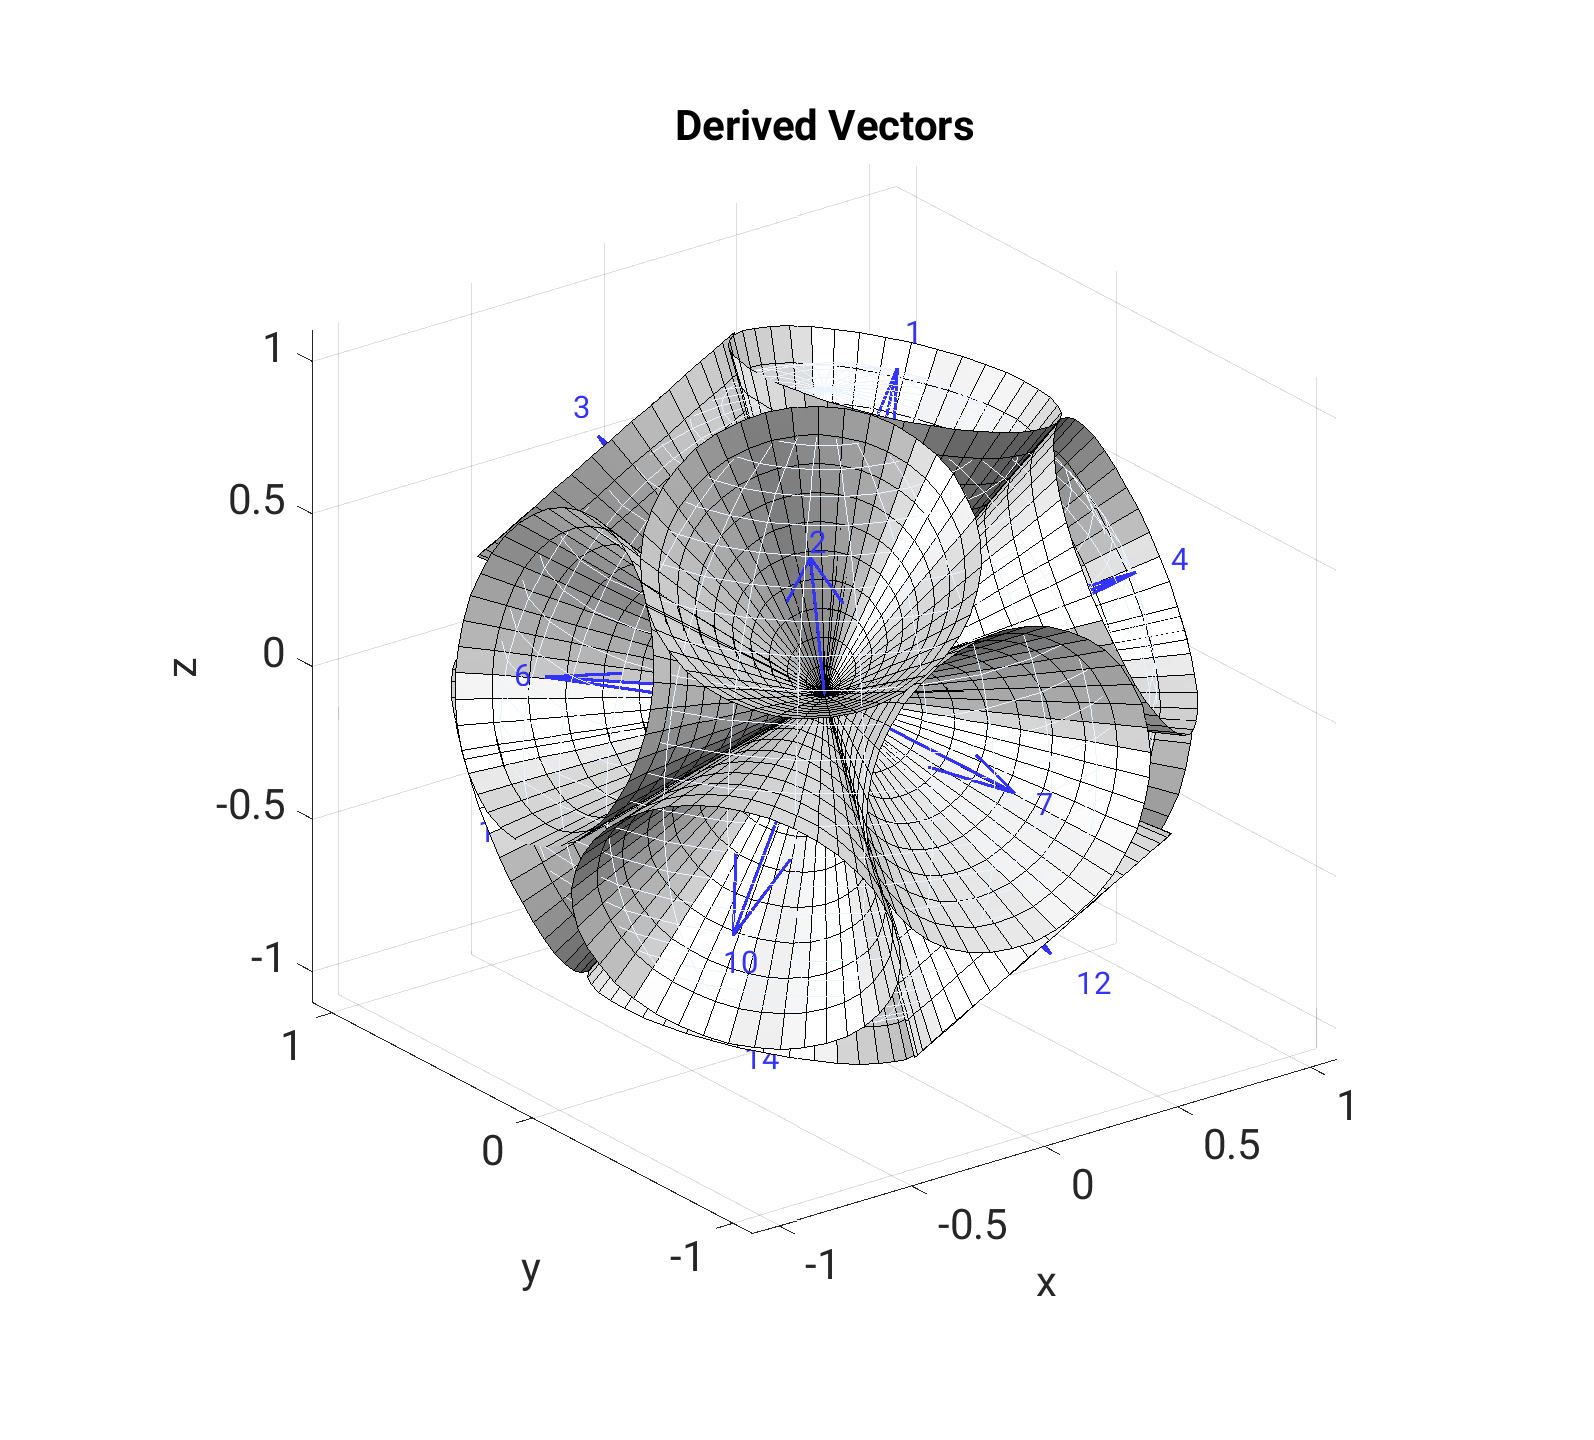
\includegraphics[width=0.8\textwidth]{Graphics/decision_cones.eps}
    \caption{Decision areas for the orthogonality threshold in 3D depicted as cones.}
    \label{figdecisioncones}
\end{figure}


Figure \ref{figdecisioncones} shows an extension of the directional vectors which were shown in in Figure \ref{vectors_from_points} on the right. For each directional vector the decision cone was plotted and it shows the boundaries of each directional vector. Each cone has the opening angle which corresponds to the angle between the first normal and the bisector between the first directional vector and its nearest neighbour. Each comparison vector which lays inside one cone would be assigned to the index of the corresponding directional vector in the middle of that cone.

\subsubsection{Assignment of directional dimensions with orthogonality threshold}

The new technique for assigning an directional index to a certain comparison vector is introduced in this section. It has some similarities to the previous angle sorting approach but differs from it in context of performance. The principle is explained with the following flowchart:

\begin{figure}[H]
    \centering
    \includegraphics[width=0.75\textwidth]{Graphics/Fringe_Orthogonality.png}
    \caption{Flowchart of the orthogonality threshold algorithm in 5D.}
    \label{ortho_threshold_flow}
\end{figure}

The input parameters for this approach are the two \textbf{comparison vectors} for both dimensions. Since the definition of the comparison vectors is free, for this example they will be defined as following: the \code{comparison\_vector4D} is defined as the vector from the voxel to receiver. The other \code{comparison\_vector5D} is defined as the vector from the voxel to the emitter.
The set of \textbf{directional vectors} that discretise the directional information of the volume are also part of the input values in form of an interleaved array of coordinates. Next the threshold value as decision criteria for each directional vector is imported. The calculation of the \textbf{orthogonality threshold} is explained in section \ref{decison_orthonolatiy}. The indices of the two directional vectors that are under investigation in that particular iteration of the reconstruction are given as  \code{current\_direction\_vector4D} and \code{current\_direction\_vector5D}. 
In the 2\textsuperscript{nd} stage of the procedure the coordinates of the directional vectors for the 4D case have to be chosen from the set of directional vectors, since \code{current\_direction\_vector4D} and \code{current\_direction\_vector5D} were only given as indices. As the coordinates of the directional vectors are interleaved in the array they can be accessed with the pointer operation that is shown in the 2\textsuperscript{nd} step of the flowchart. For '\code{+0}' the first coordinate of the directional vector is loaded. Analogously, for '\code{+1}' and '\code{+2}' the second and the third coordinates are taken from the array.
With that we have the current directional vector \code{dir\_vec4D} for that iteration.
The scalar product between the \code{comparison\_vector4D} and the directional vector \code{dir\_vec4D} is calculated in the last part of the 2\textsuperscript{nd} stage. The resulting \code{orthogonality4D} is compared to the \code{orthogonality\_threshold} which was part of the input parameters. If the \code{orthogonality4D} is smaller than the \code{orthogonality\_threshold} it can be assumed that the \code{comparison\_vector4D} does not belong to the currently investigated \code{dir\_vec4D}. In this case the algorithm will stop and continue with the next \ac{ascan} where a new \code{comparison\_vector4D} is calculated. 
If the condition leads to the conclusion that the \code{orthogonality4D} is larger than the \code{orthogonality\_threshold} the next stage of the algorithm is started.
The procedure is repeated for the 5\textsuperscript{th} dimension in the same manner leading to the \code{orthogonality5D}. If \code{orthogonality5D} actually is larger than the \code{orthogonality\_threshold} the voxel value will be assigned to the voxel position[x,y,z] and to the corresponding 4\textsuperscript{th} and 5\textsuperscript{th} dimension of the output volume. If not, the algorithm again will stop before any voxel value can be assigned to any part of the image and the next \ac{ascan} will be analysed.







\section{Performance implications of assignment approaches}
\label{Perform_eval}

In theory the voxel volume can be segmented into an arbitrary set of directions with a very high density of directional vectors. To find the corresponding vector index for each \ac{ascan} the process of index identification which is explained in section \ref{sec:index_ident} has to be repeated for every emitter-receiver combination, for each voxel and each aperture position. Furthermore, the calculation has to be repeated for each directional vector twice. Depending on which geometry or what number of $N$ particles is chosen for the generation of directional vectors, this could lead to a large amount of data that has to be processed. The average reconstruction of a three dimensional measurement volume results in

\smallskip

$\#Calculations = \#Voxel \cdot \#Emitter\cdot \#Receiver \cdot \#AperturRotation \cdot \#Vectors^2$

\smallskip
number of calculations. For the case of using a 12 faced dodecahedron, 628 emitters, 1413 receivers, a volume of 250x250x250 voxels and ten aperture positions $[12^2 \cdot 628 \cdot 1413 \cdot 250^3 \cdot 10] = 1.982x10^{16}$ calculations have to be performed to find the smallest vector index. Therefore, the performance impact of the algorithms for the identification of the index is non-negligible. By decreasing the complexity of these calculations the performance of the reconstruction algorithm can be greatly improved. The goal is to receive a qualitative performance for each iteration of the two assignment methods and to compare them on the basis of these findings.
The results of the performance analysis are presented in section \ref{performance_index_ident}.
